\documentclass{article}

% ---------------------------------------------------------------------------
% Data Science Project Report template (SoSe 2026, Chair of Machine Learning,
% Universität Regensburg). Built on the NeurIPS 2026 style file.
%
% This is a *scaffold*: each section starts with a short "guidance" comment
% distilled from the report how-to slides. Replace the TODO placeholders with
% your own content. Main text is limited to 5 pages; References, Contributions
% and the Appendix do NOT count towards that limit.
% ---------------------------------------------------------------------------

% "preprint" produces a named report (author names shown, no review line numbers,
% small "Preprint." footer). For an anonymous draft with line numbers instead,
% drop the option: \usepackage{neurips_2026}
\usepackage[preprint]{neurips_2026}

\usepackage[utf8]{inputenc} % allow utf-8 input
\usepackage[T1]{fontenc}    % use 8-bit T1 fonts
\usepackage{hyperref}       % hyperlinks
\usepackage{url}            % simple URL typesetting
\usepackage{booktabs}       % professional-quality tables
\usepackage{amsfonts}       % blackboard math symbols
\usepackage{amsmath}        % display math (align, equation, ...)
\usepackage{graphicx}       % \includegraphics
\usepackage{nicefrac}       % compact symbols for 1/2, etc.
\usepackage{microtype}      % microtypography
\usepackage{xcolor}         % colors

\title{Data Science Project Report --- \emph{your project title here}}

% List every team member. \And lets LaTeX break lines; \AND forces a break.
\author{%
  First Author \\
  Faculty of Informatics and Data Science\\
  Universität Regensburg\\
  \texttt{first.author@stud.uni-regensburg.de} \\
  % \And
  % Second Author \\
  % Faculty of Informatics and Data Science\\
  % Universität Regensburg\\
  % \texttt{second.author@stud.uni-regensburg.de} \\
}

\begin{document}

\maketitle

\begin{abstract}
  % guidance [~1 paragraph]: The abstract is optional, depending on the space
  % you have. Give a brief motivation for the problem plus a high-level summary
  % of the methodology used and the main result. One paragraph, no citations.
  TODO: one-paragraph summary --- problem, method, headline result.
\end{abstract}

\section{Introduction}
% guidance [~0.5 pages]: Explain the problem and why it matters; state your
% motivation; give the background needed and cite original sources. Be explicit
% about the input and the output, e.g.:
%   "The input to our algorithm is an {image, patient age, rainfall series, ...}.
%    We then use a {SVM, neural network, linear regression, ...} to output a
%    predicted {cancer type, stock price, shrimp population, ...}."
TODO: introduce the problem, motivation, and the input/output of your task.

\section{Related work}
% guidance [~0.5 pages, aim for >=5 references]: Find existing papers, group
% them by approach, and discuss their strengths/weaknesses and how they relate
% to your work. What is the state of the art? Useful sources: Google Scholar,
% arXiv, Semantic Scholar.
TODO: survey prior work. Cite with natbib, e.g. \citet{hastie2009elements}
proposed \dots, and similar tasks were studied by \citet{chicco2020heartfailure}.

\section{Dataset and features}
% guidance [~0.5--1 pages]: Describe the dataset (how many train/validation/test
% examples). What preprocessing did you do? Normalization or augmentation?
% Cite where the data came from. Describe the features you used and any feature
% extraction (PCA, Fourier, word2vec, HOG, ...).
TODO: describe the data, the splits, preprocessing, and the features.

\section{Methods}
% guidance [~1--1.5 pages]: Describe each learning algorithm, include the
% relevant mathematical notation, give a short (~1 paragraph) explanation of how
% it works in your own words, and justify why it suits the task/data. Example of
% a display equation (softmax over K classes):
\begin{equation}
  \operatorname{softmax}(\mathbf{z})_k = \frac{e^{z_k}}{\sum_{j=1}^{K} e^{z_j}},
  \qquad k = 1, \dots, K .
\end{equation}
TODO: describe and motivate the algorithms you chose.

\section{Results}
% guidance [~1--3 pages]: State and define your primary metrics (give equations
% where helpful), show visualizations, and discuss where/why algorithms succeed
% or fail. Discuss whether you overfit and what you did about it. Every figure
% and table must be referenced in the text (see Table~\ref{tab:results} and
% Figure~\ref{fig:results}). Example metric --- the F1 score:
\begin{equation}
  \text{F1} = 2 \cdot \frac{\text{precision} \cdot \text{recall}}
  {\text{precision} + \text{recall}} .
\end{equation}
TODO: present and discuss your results, referencing every table and figure. For instance, see Table~\ref{tab:results} and Figure~\ref{fig:results}.

\begin{table}[ht]
  \caption{Test-set performance on the synthetic heart-failure cohort
    ($n = 360$ held-out patients). All metrics lie in $[0,1]$, higher is better;
    \textbf{bold} marks the best model per column. AUC is the area under the ROC
  curve.}
  \label{tab:results}
  \centering
  \begin{tabular}{lccccc}
    \toprule
    Model               & Accuracy       & Precision      & Recall         & F1             & AUC            \\
    \midrule
    Logistic regression & 0.769          & 0.735          & 0.669          & 0.700          & 0.838          \\
    Random forest       & \textbf{0.875} & \textbf{0.862} & \textbf{0.821} & \textbf{0.841} & \textbf{0.936} \\
    Gradient boosting   & 0.869          & 0.860          & 0.807          & 0.833          & 0.919          \\
    \bottomrule
  \end{tabular}
\end{table}

\begin{figure}[ht]
  \centering
  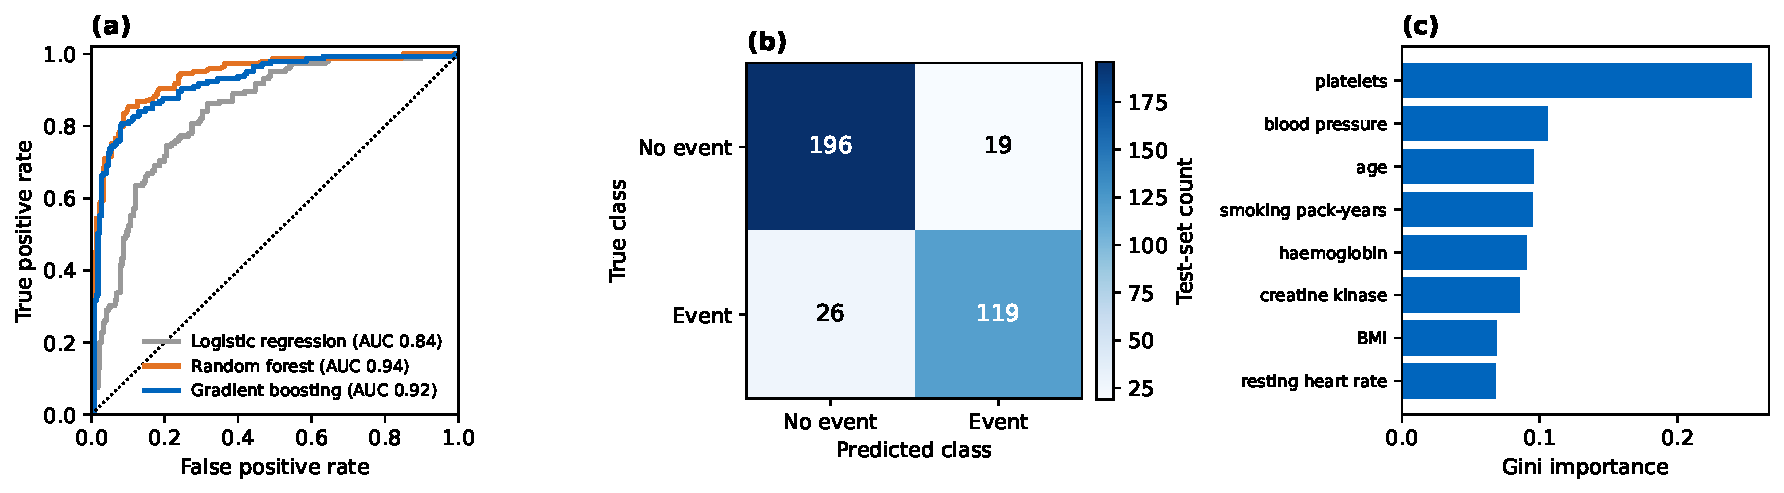
\includegraphics[width=\linewidth]{figures/example_multipanel}
  \caption{Evaluation of three classifiers on the held-out test set.
    \textbf{(a)} ROC curves; colour encodes the model and the legend reports
    each AUC. \textbf{(b)} Confusion matrix of the best model (random forest);
    cell colour and number give the test-set count. \textbf{(c)} The eight most
  important features of the random forest (Gini importance).}
  \label{fig:results}
\end{figure}

\section{Conclusion}
% guidance [~1--2 paragraphs]: Summarize the report and reiterate key points.
% Which algorithms performed best, and why do you think so? For future work:
% with more time, people, or compute, what would you explore?
TODO: summarize findings and outline future work.

\section*{Contributions}
% guidance: NOT counted in the 5-page limit. Describe what each team member
% worked on and contributed. Include contributions from Assignment 2 if relevant.
TODO: per-member contributions.

\bibliographystyle{plainnat}
\bibliography{references}

%%%%%%%%%%%%%%%%%%%%%%%%%%%%%%%%%%%%%%%%%%%%%%%%%%%%%%%%%%%%

\appendix

\section{Appendix}
% guidance: Optional and NOT counted in the 5-page limit. It must not contain
% information essential to understanding the main text. Good uses: a full table
% of hyperparameters (every value, every seed, every split), and extra figures
% or tables that are not central. Still label and reference everything.
TODO: supporting material, e.g. the hyperparameter table below.

\begin{table}[h]
  \caption{Hyperparameters used for the final models.}
  \label{tab:hyperparameters}
  \centering
  \begin{tabular}{lll}
    \toprule
    Model             & Hyperparameter & Value \\
    \midrule
    Random forest     & n\_estimators  & 300   \\
    Random forest     & random\_state  & 0     \\
    Gradient boosting & learning\_rate & 0.1   \\
    \bottomrule
  \end{tabular}
\end{table}

%%%%%%%%%%%%%%%%%%%%%%%%%%%%%%%%%%%%%%%%%%%%%%%%%%%%%%%%%%%%

\end{document}
